\section{Basic}
    \subsection{BIT}
        \lstinputlisting{Contents/basic/BIT.cpp}
    \subsection{Black Magic}
        \lstinputlisting{Contents/basic/black_magic.cpp}
    \subsection{DJS}
        \lstinputlisting{Contents/basic/disjoin_set.cpp}
    \subsection{DFS}
        \lstinputlisting{Contents/basic/DFS.cpp}
    \subsection{BFS}
        \lstinputlisting{Contents/basic/BFS.cpp}
    \subsection{segment_tree}
        \lstinputlisting{Contents/basic/segment_tree.cpp}
    \subsection{Template}
        \lstinputlisting{Contents/basic/Template.h}

\section{Data_Structure}
    \subsection{Range Sum Query}
        \lstinputlisting{Contents/data_structure/Range_Sum_Query_by_Lazy_Propagation.cpp}
    \subsection{Splay Tree}
        \lstinputlisting{Contents/data_structure/Splay_Tree.cpp}

\section{DP}
    \subsection{LCS}
        \lstinputlisting{Contents/dp/LCS.cpp}
    \subsection{LIS}
        \lstinputlisting{Contents/dp/LIS.cpp}
    \subsection{迴文}
        \lstinputlisting{Contents/dp/palindrome_in_a_string.cpp}

\section{Geometry}
    \subsection{Convex hull}
        \lstinputlisting{Contents/geometry/convex_hull.cpp}

\section{Graph}
    \subsection{Bellman Ford}
        \lstinputlisting{Contents/graph/bellman_ford.cpp}
    \subsection{Dijk}
        \lstinputlisting{Contents/graph/Dijkstra.cpp}
    \subsection{Edges}
        \lstinputlisting{Contents/graph/edge.cpp}    
    \subsection{Floyd}
        \lstinputlisting{Contents/graph/floyd.cpp}
    \subsection{KM}
        \lstinputlisting{Contents/graph/KM.cpp}
    \subsection{Global Minimum Cut}
        \lstinputlisting{Contents/graph/Global_Minimum_Cut.cpp}
    \subsection{Krushal}
        \lstinputlisting{Contents/graph/Krushal.cpp}
    \subsection{K-th Shortest Path Length}
        \lstinputlisting{Contents/graph/kth_Shortest_Path_Length.cpp}
    \subsection{SPFA}
        \lstinputlisting{Contents/graph/SPFA.cpp}

\section{Math}
    \subsection{GCDhjackh}
        \lstinputlisting{Contents/math/gcdhjackh.cpp}
    \subsection{Prime}
        \lstinputlisting{Contents/math/prime.cpp}
    \subsection{Gauss Elimination}
        \lstinputlisting{Contents/math/GaussElimination.cpp}
    \subsection{Matrix}
        \lstinputlisting{Contents/math/matrix.cpp}
        
\section{String}
    \subsection{KMP}
        \lstinputlisting{Contents/string/KMP.cpp}
    \subsection{Trie}
        \lstinputlisting{Contents/string/Trie.cpp}
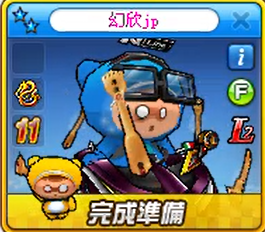
\includegraphics{Contents/runrun.png}